A performance measure is declared in the adjoint input file with one of three forms. The \emph{direct} form accumulates a quantity, the \emph{residual} form accumulates the squared difference between a quantity and an observed counterpart, and the \emph{instantaneous} form treats each observation time on its own. This chapter describes the third, and is explicit about what it does and does not answer.

\section*{What it computes}

The adjoint solution runs backward through the saved time steps, and the storage terms of Chapter~\ref{ch:storage} pass the result of one step to the step before it. A direct measure keeps that passing, so the adjoint state it reports at time step $k$ is the derivative of the accumulated measure, carrying the influence of every observation that follows.

An instantaneous measure drops it. Each observed time step is solved on its own, and a time step with no observation is not solved at all. What it reports at an observed step is the response of the measured quantity at that instant to a stress applied during that same step, at every cell in the model. Written for a head measured at cell $o$ and a rate applied at cell $c$,

\begin{equation}
	\label{eqn:inst-kernel}
	\lambda^{k}_{c} = \frac{\partial h_{o}(t_{k})}{\partial q_{c}(t_{k})},
\end{equation}

\noindent where $\lambda^{k}_{c}$ has the dimensions of a head divided by a volumetric rate (TL$^{-2}$), $h_{o}$ is the head at the measured cell (L), and $q_{c}$ is the rate applied at cell $c$ (L$^{3}$T$^{-1}$). It is a map over the model of the immediate effect of pumping. Because the steps are solved independently, this map does not change when other observation times are added to the same measure.

The measure value itself is the time-weighted mean of the observed steps,

\begin{equation}
	\label{eqn:instantaneous}
	J_{\mathrm{inst}} = \frac{\sum_{k} \Delta t^{k} F^{k}}{\sum_{k} \Delta t^{k}},
\end{equation}

\noindent rather than the sum equation~\ref{eqn:pm} gives.

\section*{Where it agrees with a direct measure}

The two forms differ only where there is something to pass backward, which gives two cases in which they agree exactly.

A steady-state time step has no storage, so nothing is carried and the question a direct measure asks is already the question an instantaneous measure asks. The last time step solved agrees for the same reason: the adjoint begins there, so nothing has fed back into it yet.

Figure~\ref{fig:instantaneous} shows both. The sensitivity of a head to a well rate was computed with each form on a model whose first stress period is steady state and whose remaining five are transient, with an observation at every time step. The two agree through the steady period and again at the final step, and differ at the twenty transient steps between them, where the direct form carries the influence of the later observations and the instantaneous form does not.

\begin{figure}[htb]
	\centering
	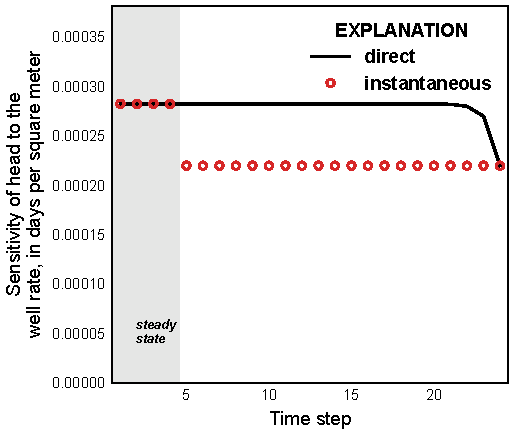
\includegraphics{Figures/instantaneous.pdf}
	\caption{Sensitivity of head at an observation cell to the rate of a well, computed as a direct measure and as an instantaneous measure, for a model whose first stress period is steady state (shaded) and whose remaining periods are transient. Both forms carry an observation at every time step. The two agree at the four steady-state steps and at the last step solved, and differ at the transient steps between them.}
	\label{fig:instantaneous}
\end{figure}

\section*{What it is for}

The map of equation~\ref{eqn:inst-kernel} answers a question about the present: where does a stress applied now have the most effect on the measured quantity now. Held against a stream or a lake, it locates the cells whose pumping is felt immediately by that boundary, which is the quantity a short-horizon management problem is written in terms of. It is also inexpensive, because only the observed steps are solved: a measure observed at one time in a two hundred step simulation costs one solve rather than two hundred.

The independence of the observed steps is the other reason to prefer it. Every entry of an instantaneous measure reports the same map it would report alone, so the entries of one measure can be read as separate answers. The entries of a direct measure cannot, because each carries the influence of those after it.

\section*{What it is not for}

An instantaneous measure does not give the response of the measured quantity to a stress applied at an earlier time. That response is what makes drawdown deepen while a well runs, and it is carried by exactly the passing between time steps that this form drops. Adding the maps of successive steps together does not recover it, because each map reports the effect of a stress applied within its own step and none of them reports the effect that stress continues to have afterward.

The consequence is worth stating plainly, because the sum is a natural thing to try. Accumulated over a simulation in which a well pumps at a constant rate, the maps grow the drawdown linearly with the number of steps, while the drawdown of a confined aquifer grows with the logarithm of time. The accumulation is therefore exact after the first time step, where there is no earlier stress to account for, and departs from the simulated drawdown thereafter.

A measure whose answer depends on the history of the stresses, including drawdown through time and the response matrix that reconstructs it, needs the direct form.
